\documentclass[border=15pt, multi, tikz]{standalone}
\usepackage{import}
\subimport{./layers/}{init}
\usetikzlibrary{positioning}
\usetikzlibrary{3d} % for including external image

% Layer colors
\def\ConvColor{rgb:yellow,5;red,2.5;white,5}
\def\ConvReluColor{rgb:yellow,5;red,5;white,5}
\def\PoolColor{rgb:red,1;black,0.3}
\def\DcnvColor{rgb:blue,5;green,2.5;white,5}
\def\SoftmaxColor{rgb:magenta,5;black,7}
\def\FcColor{rgb:blue,5;black,5}

\begin{document}
\begin{tikzpicture}
\tikzstyle{connection}=[ultra thick,every node/.style={sloped,allow upside down},draw=black,opacity=0.7]

%%%%%%%%%%%%%%%%%%%%%%%%%%%%%%%%%%%%%%%%%%%%%%%%%%%%%%%%%%%%%%%%%%%%%%%%%%%%%%%%%%%%%%%%
%% Optional: input image
%%%%%%%%%%%%%%%%%%%%%%%%%%%%%%%%%%%%%%%%%%%%%%%%%%%%%%%%%%%%%%%%%%%%%%%%%%%%%%%%%%%%%%%%
\node[canvas is zy plane at x=0 , xscale=-1] (inputimg) at (-1,0,0) {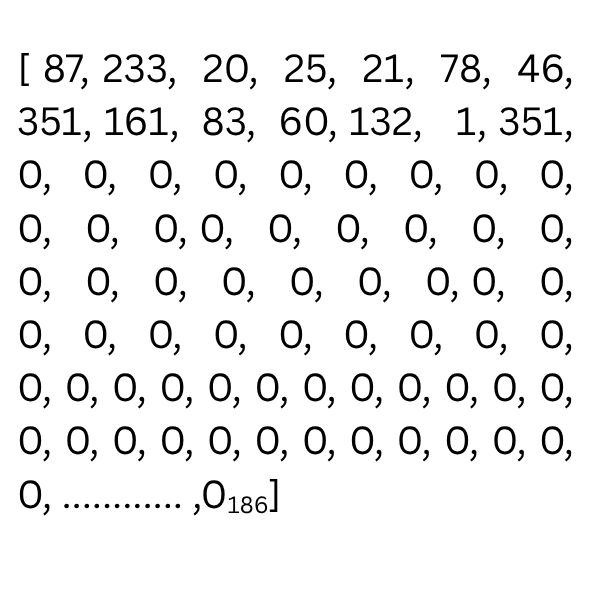
\includegraphics{./input.jpg}};

%%%%%%%%%%%%%%%%%%%%%%%%%%%%%%%%%%%%%%%%%%%%%%%%%%%%%%%%%%%%%%%%%%%%%%%%%%%%%%%%%%%%%%%%
%% Model layers
%%%%%%%%%%%%%%%%%%%%%%%%%%%%%%%%%%%%%%%%%%%%%%%%%%%%%%%%%%%%%%%%%%%%%%%%%%%%%%%%%%%%%%%%

% Embedding
\pic[shift={(0,0,0)}] at (0,0,0) {RightBandedBox={
    name=embedding,
    caption={{\\Embedding Layer}},
    xlabel={{"","None X 186 X 190",""}}, 
    fill=\ConvColor, bandfill=\ConvReluColor,
    height=28, width={3,3,3}, depth=28
}};
% Conv1D
\pic[shift={(2.5,0,0)}] at (embedding-east) {Box={
    name=Conv1D,
    caption={{\\Conv1D Layer}},
    xlabel={{"","128",""}}, 
    fill=\SoftmaxColor,
    height=24,width={4,4},depth=20
}};

% GlobalMaxPooling1D
\pic[shift={(2,0,0)}] at (Conv1D-east) {Box={
    name=GlobalMaxPooling1D,
    caption={{\\GlobalMaxPooling1D Layer}},
    xlabel={{"","",""}}, 
    fill=\ConvReluColor,
    height=24,width={5},depth=20
}};

% Dense Layer
\pic[shift={(2,0,0)}] at (GlobalMaxPooling1D-east) {Box={
    name=dense1,
    caption={{\\Dense Layer}},
    xlabel={{"24","24",""}},
    fill=\DcnvColor,
    height=16,width=3,depth=20
}};


% Dense Layer
\pic[shift={(2,0,0)}] at (dense1-east) {Box={
    name=dense,
    caption={{\\Softmax Layer}},
    xlabel={{"","2",""}}, zlabel= output,
    fill=\FcColor,
    height=8,width=1,depth=8
}};

% LIME
\pic[shift={(2.5,0,0)}] at (dense-east) {Box={name=d16,%
        xlabel={{"","dummy"}},fill=\DcnvColor,opacity=0.7,height=20,width=0.5,depth=20}};
%% Dcnv8    
\pic[shift={(.25,0,0)}] at (d16-east) {Box={name=d8,%
        xlabel={{"","dummy"}},fill=\DcnvColor,opacity=0.7,height=20,width=0.5,depth=20}};
%% Dcnv4    
\pic[shift={(.25,0,0)}] at (d8-east) {Box={name=d4,%
        xlabel={{"","dummy"}},fill=\DcnvColor,opacity=0.7,height=20,width=0.5,depth=20}};
%% Dcnv2    
\pic[shift={(.25,0,0)}] at (d4-east) {Box={name=d2,%
        xlabel={{"","dummy"}},fill=,opacity=0.01,height=20,width=0.5,depth=20}};

%% Dcnv envelope    
\pic[shift={(-0.2,0,0)}] at (d16-west) {Box={name=env,caption=LIME,%
        xlabel={{"","dummy"}},fill=,opacity=0.2,height=22,width={8},depth=22}};

\node[canvas is zy plane at x=0, xscale=-1] (outputimg) at (20,0,0) {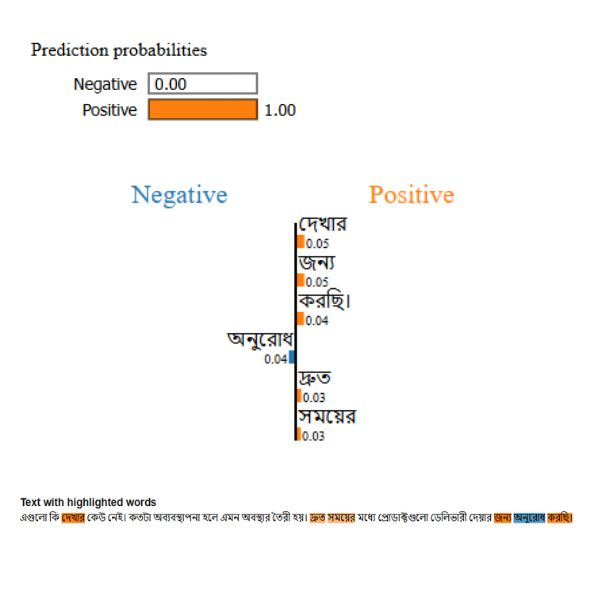
\includegraphics[width=8cm,height=8cm]{./output.jpg}};

%%%%%%%%%%%%%%%%%%%%%%%%%%%%%%%%%%%%%%%%%%%%%%%%%%%%%%%%%%%%%%%%%%%%%%%%%%%%%%%%%%%%%%%%
%% Connections
%%%%%%%%%%%%%%%%%%%%%%%%%%%%%%%%%%%%%%%%%%%%%%%%%%%%%%%%%%%%%%%%%%%%%%%%%%%%%%%%%%%%%%%%

\draw [connection] (embedding-east) -- node {\midarrow} (Conv1D-west);
\draw [connection] (Conv1D-east) -- node {\midarrow} (GlobalMaxPooling1D-west);
\draw [connection] (GlobalMaxPooling1D-east) -- node {\midarrow} (dense1-west);
\draw [connection] (dense1-east) -- node {\midarrow} (dense-west);
% \draw [connection] (Conv1D-east) -- node {\midarrow} (dense-west);

\draw[densely dashed]
(dense-east) -- (env-nearnorthwest)
(dense-east) -- (env-nearsouthwest)
(dense-east)  -- (env-farsouthwest)
(dense-east)  -- (env-farnorthwest)
;

\end{tikzpicture}
\end{document}
